 \documentclass{beamer}
%
% Choose how your presentation looks.
% For more themes, color themes and font themes, see:
% http://deic.uab.es/~iblanes/beamer_gallery/index_by_theme.html
%
\mode<presentation>
{
  \usetheme{Madrid}      % or try Darmstadt, Madrid, Warsaw, ...
  \usecolortheme{seahorse} % or try albatross, beaver, crane, ...
  \usefonttheme{serif}  % or try serif, structurebold, ...
  \setbeamertemplate{navigation symbols}{}
  \setbeamertemplate{caption}[numbered]
  \usepackage{amsmath}
  \usepackage{tcolorbox}
  \usepackage[export]{adjustbox}
  \tcbuselibrary{most}
  \usepackage{arydshln}
  \usepackage{tikz}
  \usetikzlibrary{plotmarks}
  \usepackage{pgfplots}
 %\usepackage{enumitem}
%\usepackage{enumerate}
  %\usepackage[shortlabels]{enumitem}
} 


\definecolor{myblue}{RGB}{65,105,225} 
\definecolor{myorange}{RGB}{250,190,0}

\setbeamercolor{structure}{fg=white,bg=myorange}
\setbeamercolor*{palette primary}{fg=myblue,bg=myorange}
\setbeamercolor*{palette secondary}{fg=white,bg=myblue}
\setbeamercolor*{palette tertiary}{bg=myblue,fg=white}
\setbeamercolor*{palette quaternary}{fg=white,bg=myorange!50}

\setbeamercolor{frametitle}{fg=black!90!myblue}

\setbeamercolor{section in head/foot}{fg=white,bg=myblue}
\setbeamercolor{author in head/foot}{fg=black,bg=myorange}
\setbeamercolor{title in head/foot}{fg=white,bg=myblue}

\setbeamertemplate{navigation symbols}{}

\setbeamertemplate{itemize/enumerate body begin}{\large}
\setbeamertemplate{itemize/enumerate subbody begin}{\large}


\defbeamertemplate*{headline}{mytheme}
{%
  \begin{beamercolorbox}[ht=2.25ex,dp=3.75ex]{section in head/foot}
    \insertnavigation{\paperwidth}
  \end{beamercolorbox}%
}%

\defbeamertemplate*{footline}{mytheme}
{
  \leavevmode%
  \hbox{%
  \begin{beamercolorbox}[wd=.5\paperwidth,ht=2.25ex,dp=1ex,right]{author in head/foot}%
    \usebeamerfont{author in head/foot}\insertshortauthor\hspace*{2em}
  \end{beamercolorbox}%
  \begin{beamercolorbox}[wd=.5\paperwidth,ht=2.25ex,dp=1ex,left]{title in head/foot}%
    \usebeamerfont{title in head/foot}\hspace*{2em}\insertshortsubtitle\hspace*{2em}
    \insertframenumber{} / \inserttotalframenumber
  \end{beamercolorbox}}%
  \vskip0pt%
}

\usepackage[english]{babel}
%\usepackage[utf8x]{inputenc}
\usepackage{xcolor}
\usepackage{listings}
\usepackage{pgf}  
\usepackage{textpos}
\usepackage{tabulary}
\usepackage{scrextend}
\usepackage{hyperref}
\usepackage{setspace}
\usepackage{rotating}
\lstset
{
    language=[LaTeX]TeX,
    breaklines=true,
    basicstyle=\tt\scriptsize,
    %commentstyle=\color{green}
    keywordstyle=\color{blue},
    %stringstyle=\color{black}
    identifierstyle=\color{magenta},
}
\newcommand{\bftt}[1]{\textbf{\texttt{#1}}}
%\newcommand{\comment}[1]{{\color[HTML]{008080}\textit{\textbf{\texttt{#1}}}}}
\newcommand{\cmd}[1]{{\color[HTML]{008000}\bftt{#1}}}
\newcommand{\bs}{\char`\\}
\newcommand{\cmdbs}[1]{\cmd{\bs#1}}
\newcommand{\lcb}{\char '173}
\newcommand{\rcb}{\char '175}
\newcommand{\cmdbegin}[1]{\cmdbs{begin\lcb}\bftt{#1}\cmd{\rcb}}
\newcommand{\cmdend}[1]{\cmdbs{end\lcb}\bftt{#1}\cmd{\rcb}}

\newcommand{\wllogo}{\textbf{Overleaf}}

% this is where the example source files are loaded from
% do not include a trailing slash
\newcommand{\fileuri}{https://raw.githubusercontent.com/GiancarloSucci/UniBo.IDSEPC.A2022/main/A2022.IDSEPCLaTeX/}


\usepackage{stackengine}
\def\Ruble{\stackengine{.67ex}{%
  \stackengine{.48ex}{\textsf{P}}{\rule{.8ex}{.12ex}\kern.6ex}{O}{r}{F}{F}{L}%
  }{\rule{.8ex}{.12ex}\kern.6ex}{O}{r}{F}{F}{L}\kern-.1ex}



%----------------------------------------------------------------------------------------
%	TITLE PAGE
%----------------------------------------------------------------------------------------
\title[L04]{Artificial Intelligence, Blockchain, e Criptovalute nello Sviluppo Software \newline\newline
Lezione 4: Cognitive Models in Software Development -- Measuring brain signals} % The short title appears at the bottom of every slide, the full title is only on the title page

\author[{\tiny Giancarlo Succi }]{Giancarlo Succi\\\\ Dipartimento di Informatica -- Scienza e Ingegneria\\Universit\`{a} di Bologna\\
\bftt{g.succi@unibo.it}
} % Your name
\institute[unibo] % Your institution as it will appear on the bottom of every slide, may be shorthand to save space


\date{} % Date, can be changed to a custom date

\setbeamertemplate{navigation symbols}{}
\AtBeginSection[]
{
        \begin{frame}<beamer>{Outline}
                \tableofcontents[currentsection]
        \end{frame}
}
\begin{document}
\begin{frame}
\titlepage % Print the title page as the first slide

\end{frame}

%=============================================

\addtobeamertemplate{frametitle}{}{%
\begin{textblock*}{10mm}(-0.01mm,-0.95cm)

\includegraphics[width=0.9cm]{unibo-logo.png}
\end{textblock*}}

%=============================================


\begin{frame}
{\centerline{Sources}}
\begin{itemize}
    \item This presentation has been elaborated  based on these sources and customized for the needs of this presentation:
    \begin{itemize}
        \item  A. Gramfort, M. Luessi, E. Larson, D. A. Engemann, D. Strohmeier, C.Brodbeck, R. Goj, M. Jas, T. Brooks, L. Parkkonen,et al., ``MEG and EEG data analysis with MNE-python,'' Frontiers in neuroscience, vol. 7, p. 267,2013
        \item A. Gramfort, M. Luessi, E. Larson, D. A. Engemann, D. Strohmeier, C.Brodbeck, L. Parkkonen, and M. S. H\"{a}m\"{a}l\"{a}inen, ``MNE software for processing MEG and EEG data,'' Neuroimage, vol. 86, pp. 446–460, 2014.
        \item J.-M. Schoffelen and J. Gross, ``Source connectivity analysis with MEG and EEG,'' Human brain mapping, vol. 30, no. 6, pp. 1857–1865, 2009.
    \end{itemize}
\end{itemize}
\end{frame}

\begin{frame}
{\centerline{Sources}}
\begin{itemize}
\begin{itemize}
    \item W. Klimesch, M. Doppelmayr, T. Pachinger, and B. Ripper, ``Brain oscillations  and  human  memory:  EEG  correlates  in  the  upper  alpha  and  theta band,'' Neuroscience letters, vol. 238, no. 1-2, pp. 9–12, 1997.
    \item  I. Crk, T. Kluthe, and A. Stefik ``Understanding programming expertise:An empirical study of phasic brain wave changes,''  ACM Transactions on Computer-Human Interaction (TOCHI), vol. 23, no. 1, pp. 1–29, 2015
    \item \href{https://en.wikipedia.org/wiki/10\%5C\%E2\%5C\%80\%5C\%9320_system_(EEG).}{Wikipedia} - 10–20  system  (EEG)
\end{itemize}
\item The team composing them included Sergei Bakaleinik (main writer), Sara Busechian, Gcinizwe Dlamini, and Giancarlo Succi
\end{itemize}

\end{frame}


\begin{frame}
{\centerline{Content}}
\begin{itemize}
    \item Concept of brain signals
    \item From nervous system to senses
    \item Kind of brain signals
    \item Measuring Brain Signals
    \item Inferring mental states from brain signals
    \item From frequencies to brainwave names
    \item Sample of situations,explained by brainwaves
    \item Collecting brain signals using EEG
    \item EEG software and device that we use
    \item Understanding the output of EEG
    \item Steps in the processing of EEG data
    \item About the MNE
    \item Steps undertaken in Python to analyse data from EEG
    \item Main techniques in EEG analyzing
\end{itemize}
\end{frame}


%------------------------------------------------
\begin{frame}
{\centerline{Concept of brain signals}}

\begin{figure}
    \centering
    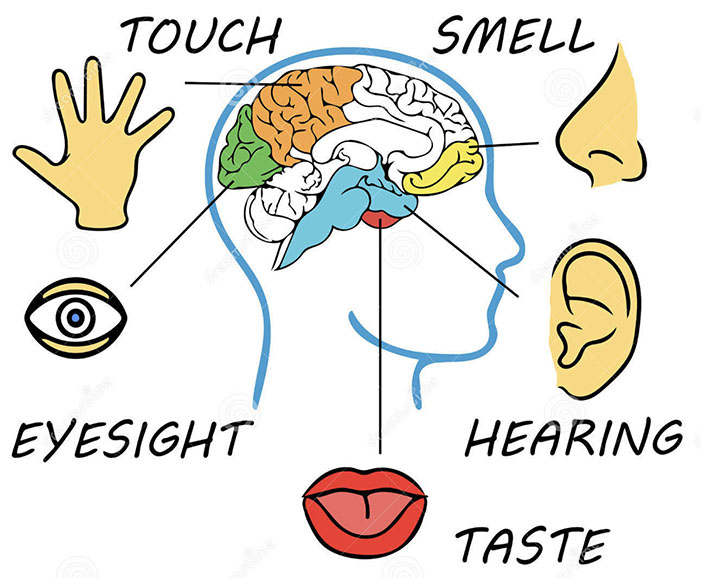
\includegraphics[height=5cm]{P2023.AIBCCSS.BrainSignals/5Senses.jpg}
    \caption{Senses to brain lobes}
\end{figure}

\begin{center}
    \tiny{Taken from \url{http://udel.edu/~livcar/Art205/Project\%202/}}
\end{center}    

\end{frame}

\begin{frame}
{\centerline{Concept of brain signals}}
\begin{itemize}
    \item The brain is the main component of the nervous system. 
    \item It is responsible for all mental operations such as concentration, thinking, learning, and motor control.
    \item These capabilities are implemented through neurons.
    \item  Our brain produces many messages to the body in the form of electrical or chemical signals.
    \item Electrical signals are also so called ``brain waves.''
    \item From the Wikipedia:
    \begin{quote}
        Neural oscillations, or brainwaves, are rhythmic or repetitive patterns of neural activity in the central nervous system.
    \end{quote}
\end{itemize}

\begin{center}
    \tiny{Taken from \url{https://en.wikipedia.org/wiki/Neural_oscillation}}
\end{center}    

\end{frame}



\begin{frame}
{\centerline{From nervous system to senses (1/3)}}
\begin{itemize}
    \item \textbf{Sight} : Light which entering the eye forms an inverted image on the retina. The light activates receptors on the retina, and those convert light to nerve signals.
\end{itemize}
\begin{figure}
    \centering
    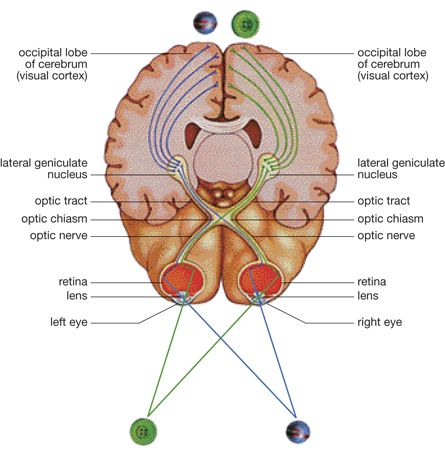
\includegraphics[height=4cm]{P2023.AIBCCSS.BrainSignals/sight.jpg}
\end{figure}
\begin{center}
    \tiny{Taken from \url{https://theconversation.com/curious-kids-how-does-our-brain-send-signals-to-our-body-124950}}
    \tiny{Image taken from \url{https://www.pinterest.ca/pin/381539399665835505/}}
\end{center}    
\end{frame}

\begin{frame}
{\centerline{From nervous system to senses (2/3)}}
\begin{itemize}
    \item \textbf{Hearing} : Every sound we hear is the result of sound waves entering our ears and causing our tympanic membrane to vibrate. These vibrations are converted into nerve signals and the cerebral cortex processes electrical signals.
\end{itemize}
\begin{figure}
    \centering
    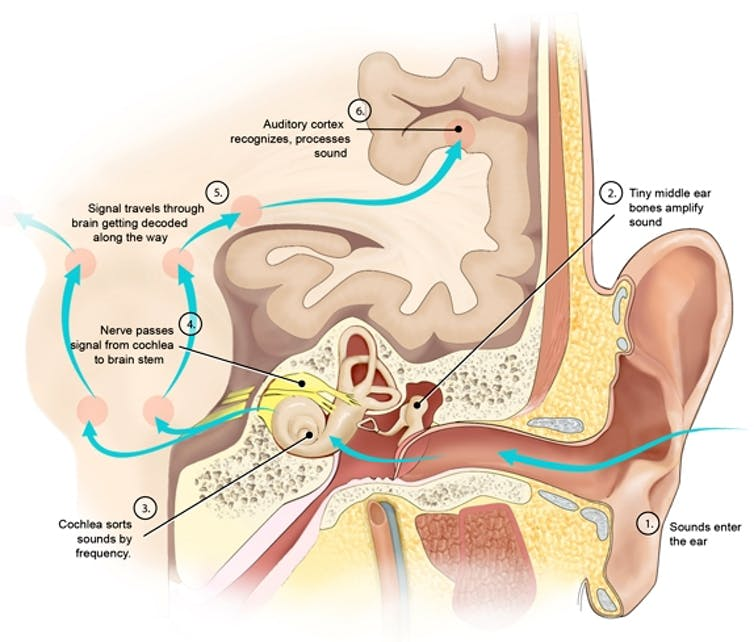
\includegraphics[height=4cm]{P2023.AIBCCSS.BrainSignals/hearing.jpg}
\end{figure}
\begin{center}
    \tiny{Taken from \url{https://theconversation.com/curious-kids-how-does-our-brain-send-signals-to-our-body-124950}}
    \tiny{Image taken from \url{https://theconversation.com/your-next-hearing-aid-could-be-a-video-game-89218}}
\end{center}    
\end{frame}


\begin{frame}
{\centerline{From nervous system to senses (3/3)}}
\begin{itemize}
    \item \textbf{Smell} : When smell molecules enter the nose, they break down and bind to olfactory receptors, which are activated and send signals through the olfactory nerve to the brain.
\end{itemize}
\begin{figure}
    \centering
    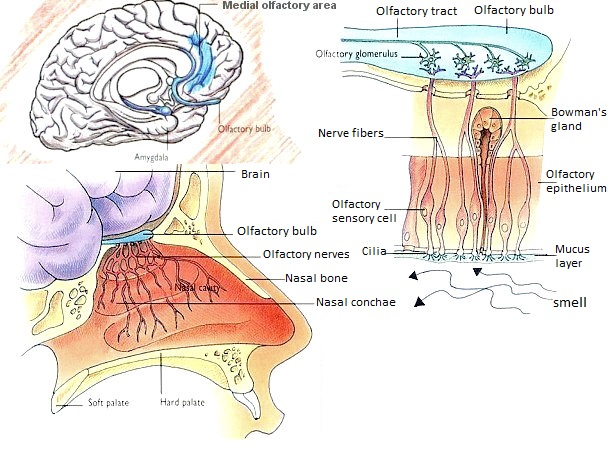
\includegraphics[height=4cm]{P2023.AIBCCSS.BrainSignals/smell.jpg}
\end{figure}
\begin{center}
    \tiny{Taken from \url{https://theconversation.com/curious-kids-how-does-our-brain-send-signals-to-our-body-124950}}
    \tiny{Image taken from \url{https://universe-review.ca/R10-16-ANS06.htm\#smell}}
\end{center}    

\end{frame}


\begin{frame}
{\centerline{Kind of brain signals}}
\begin{itemize}
    \item Brain signals have a different nature:
    \begin{itemize}
        \item electrical,
        \item chemical.
    \end{itemize}
\end{itemize}

For example: smell, convert chemical to electrical signals; sight send electrical signals to brain.

\end{frame}

\begin{frame}
{\centerline{Measuring Brain Signals (1/10)}}
    \begin{figure}
        \centering
        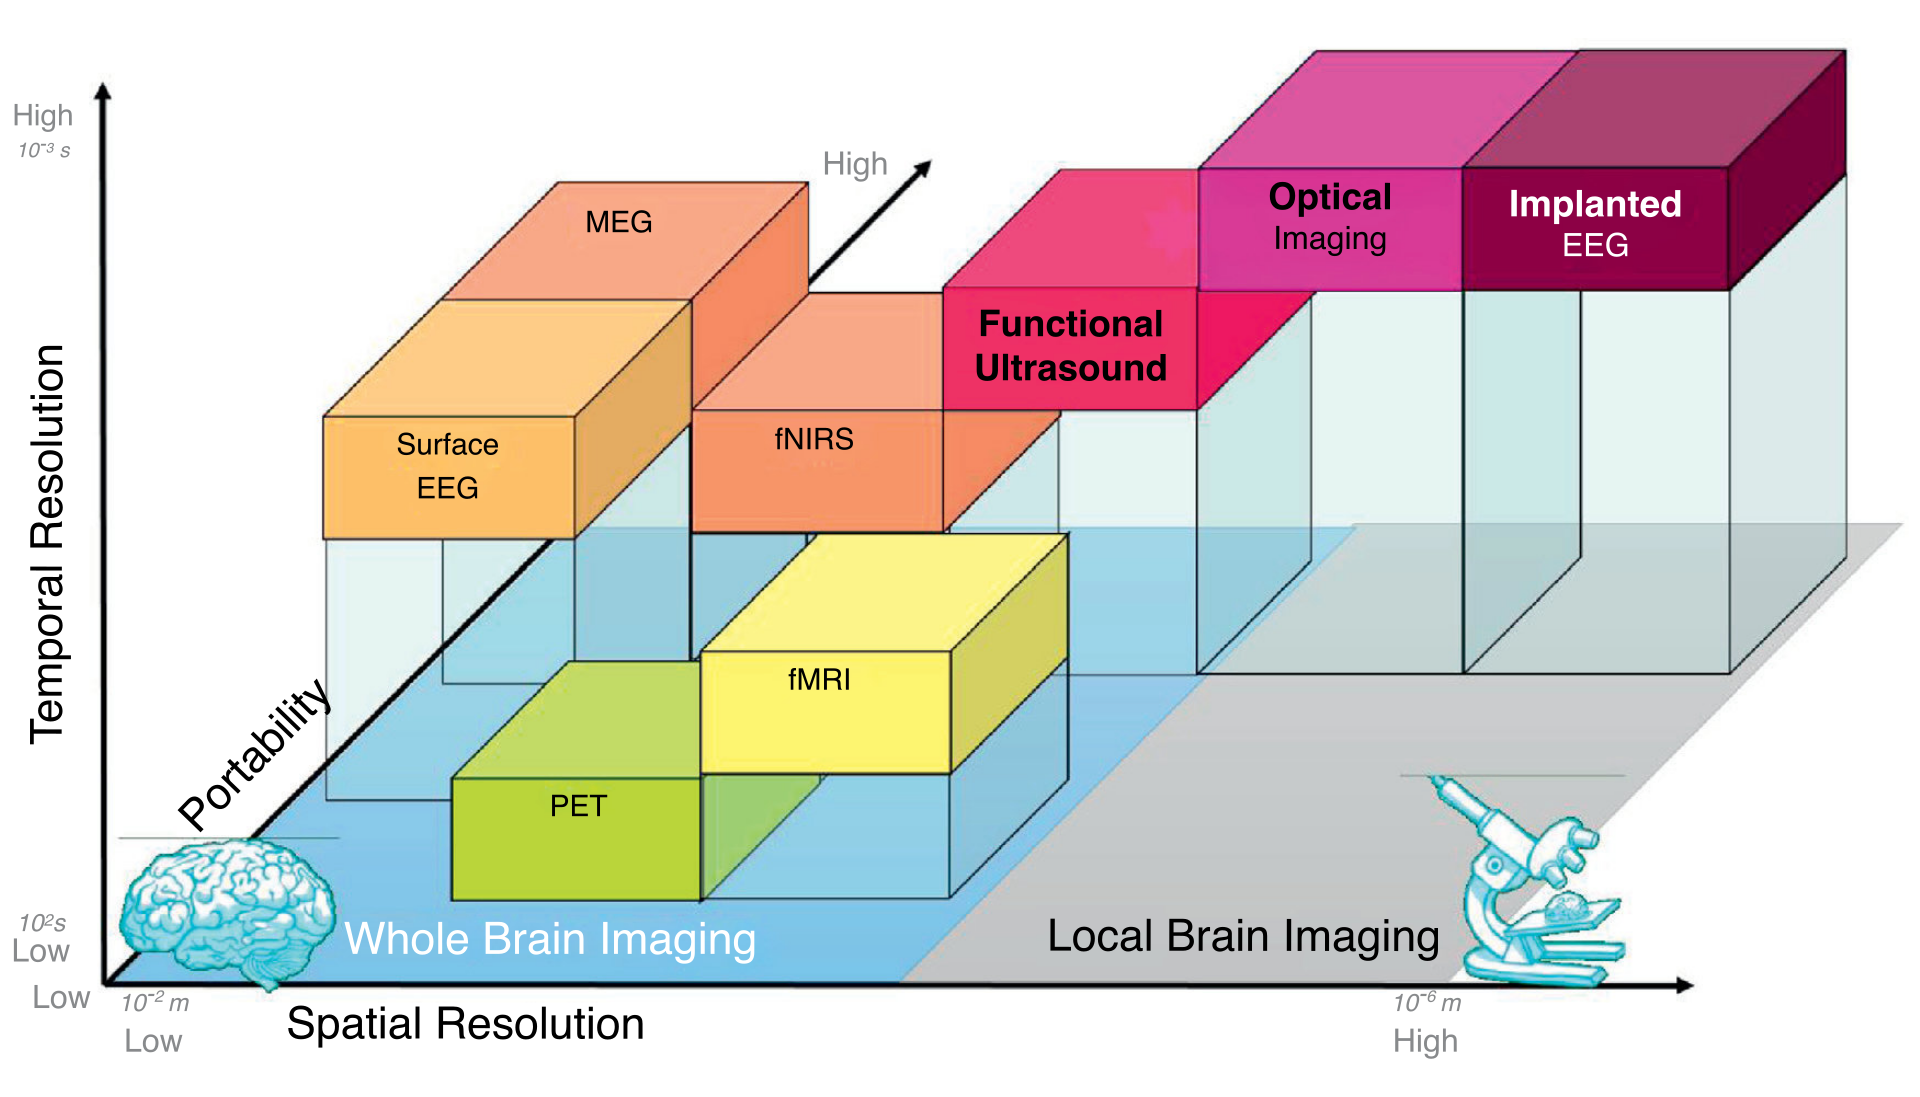
\includegraphics[height=6cm]{P2023.AIBCCSS.BrainSignals/1920px-Main_brain_functional_imaging_technique_resolutions.svg.png}
    \end{figure}
    \begin{center}
    \tiny{Taken from \url{https://en.wikipedia.org/wiki/Functional_neuroimaging}}
    \end{center} 
\end{frame}

\begin{frame}
{\centerline{Measuring Brain Signals (2/10)}}
In this presentation we more focus on electric waves. Common methods of functional neuroimaging include next devices (techniques):
\begin{itemize}
    \item Electroencephalography (EEG)
    \item Magnetoencephalography (MEG)
    \item Positron emission tomography (PET)
    \item Functional magnetic resonance imaging (fMRI)
    \item Functional near-infrared spectroscopy (fNIRS)
    \item Single-photon emission computed tomography (SPECT)
    \item Functional ultrasound imaging (fUS)
\end{itemize}
   \begin{center}
    \tiny{Taken from \url{https://en.wikipedia.org/wiki/Functional_neuroimaging}}
    \end{center} 
\end{frame}

\begin{frame}
{\centerline{Measuring Brain Signals (3/10)}}
\begin{itemize}
    \item  PET, fMRI, fNIRS, and fUS can measure localized changes in cerebral blood flow related to neural activity.
    \item Regions of the brain which are activated when a subject performs a particular task.
    \item Other methods of neuroimaging involve the recording of electrical currents or magnetic fields, for example EEG and MEG.
    \item MEG measures brain activity with high temporal resolution, but is limited in its ability to localize that activity
    \item fMRI does a much better job of localizing brain activity for spatial resolution, but with a much lower time resolution
    \item fUS can reach an interesting spatio-temporal resolution but is also limited by the neurovascular coupling
\end{itemize}
    \begin{center}
    \tiny{Taken from \url{https://en.wikipedia.org/wiki/Functional_neuroimaging}}
    \end{center}
\end{frame}

\begin{frame}
{\centerline{Measuring Brain Signals (4/10)}}
\begin{itemize}
    \item Electroencephalography (EEG)
\end{itemize}
\begin{figure}
    \centering
    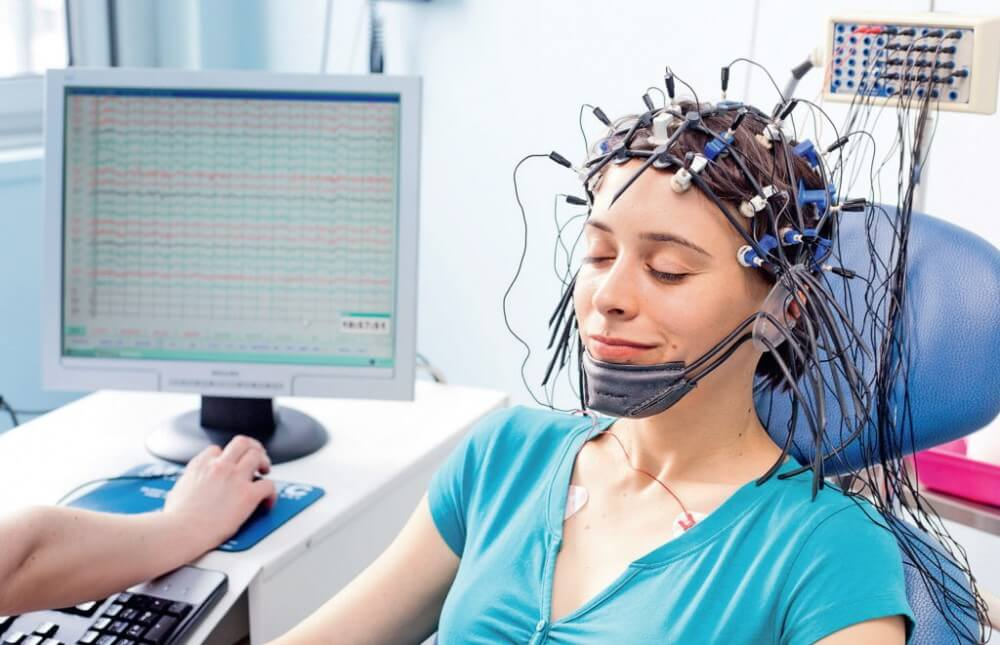
\includegraphics[height=6cm]{P2023.AIBCCSS.BrainSignals/EEG.jpg}
\end{figure}
\begin{center}
    \tiny{Taken from \url{https://tebmedtourism.com/eeg/}}
\end{center}    
\end{frame}

\begin{frame}
{\centerline{Measuring Brain Signals (5/10)}}
\begin{itemize}
    \item Magnetoencephalography (MEG)
\end{itemize}
\begin{center}

\begin{figure}
    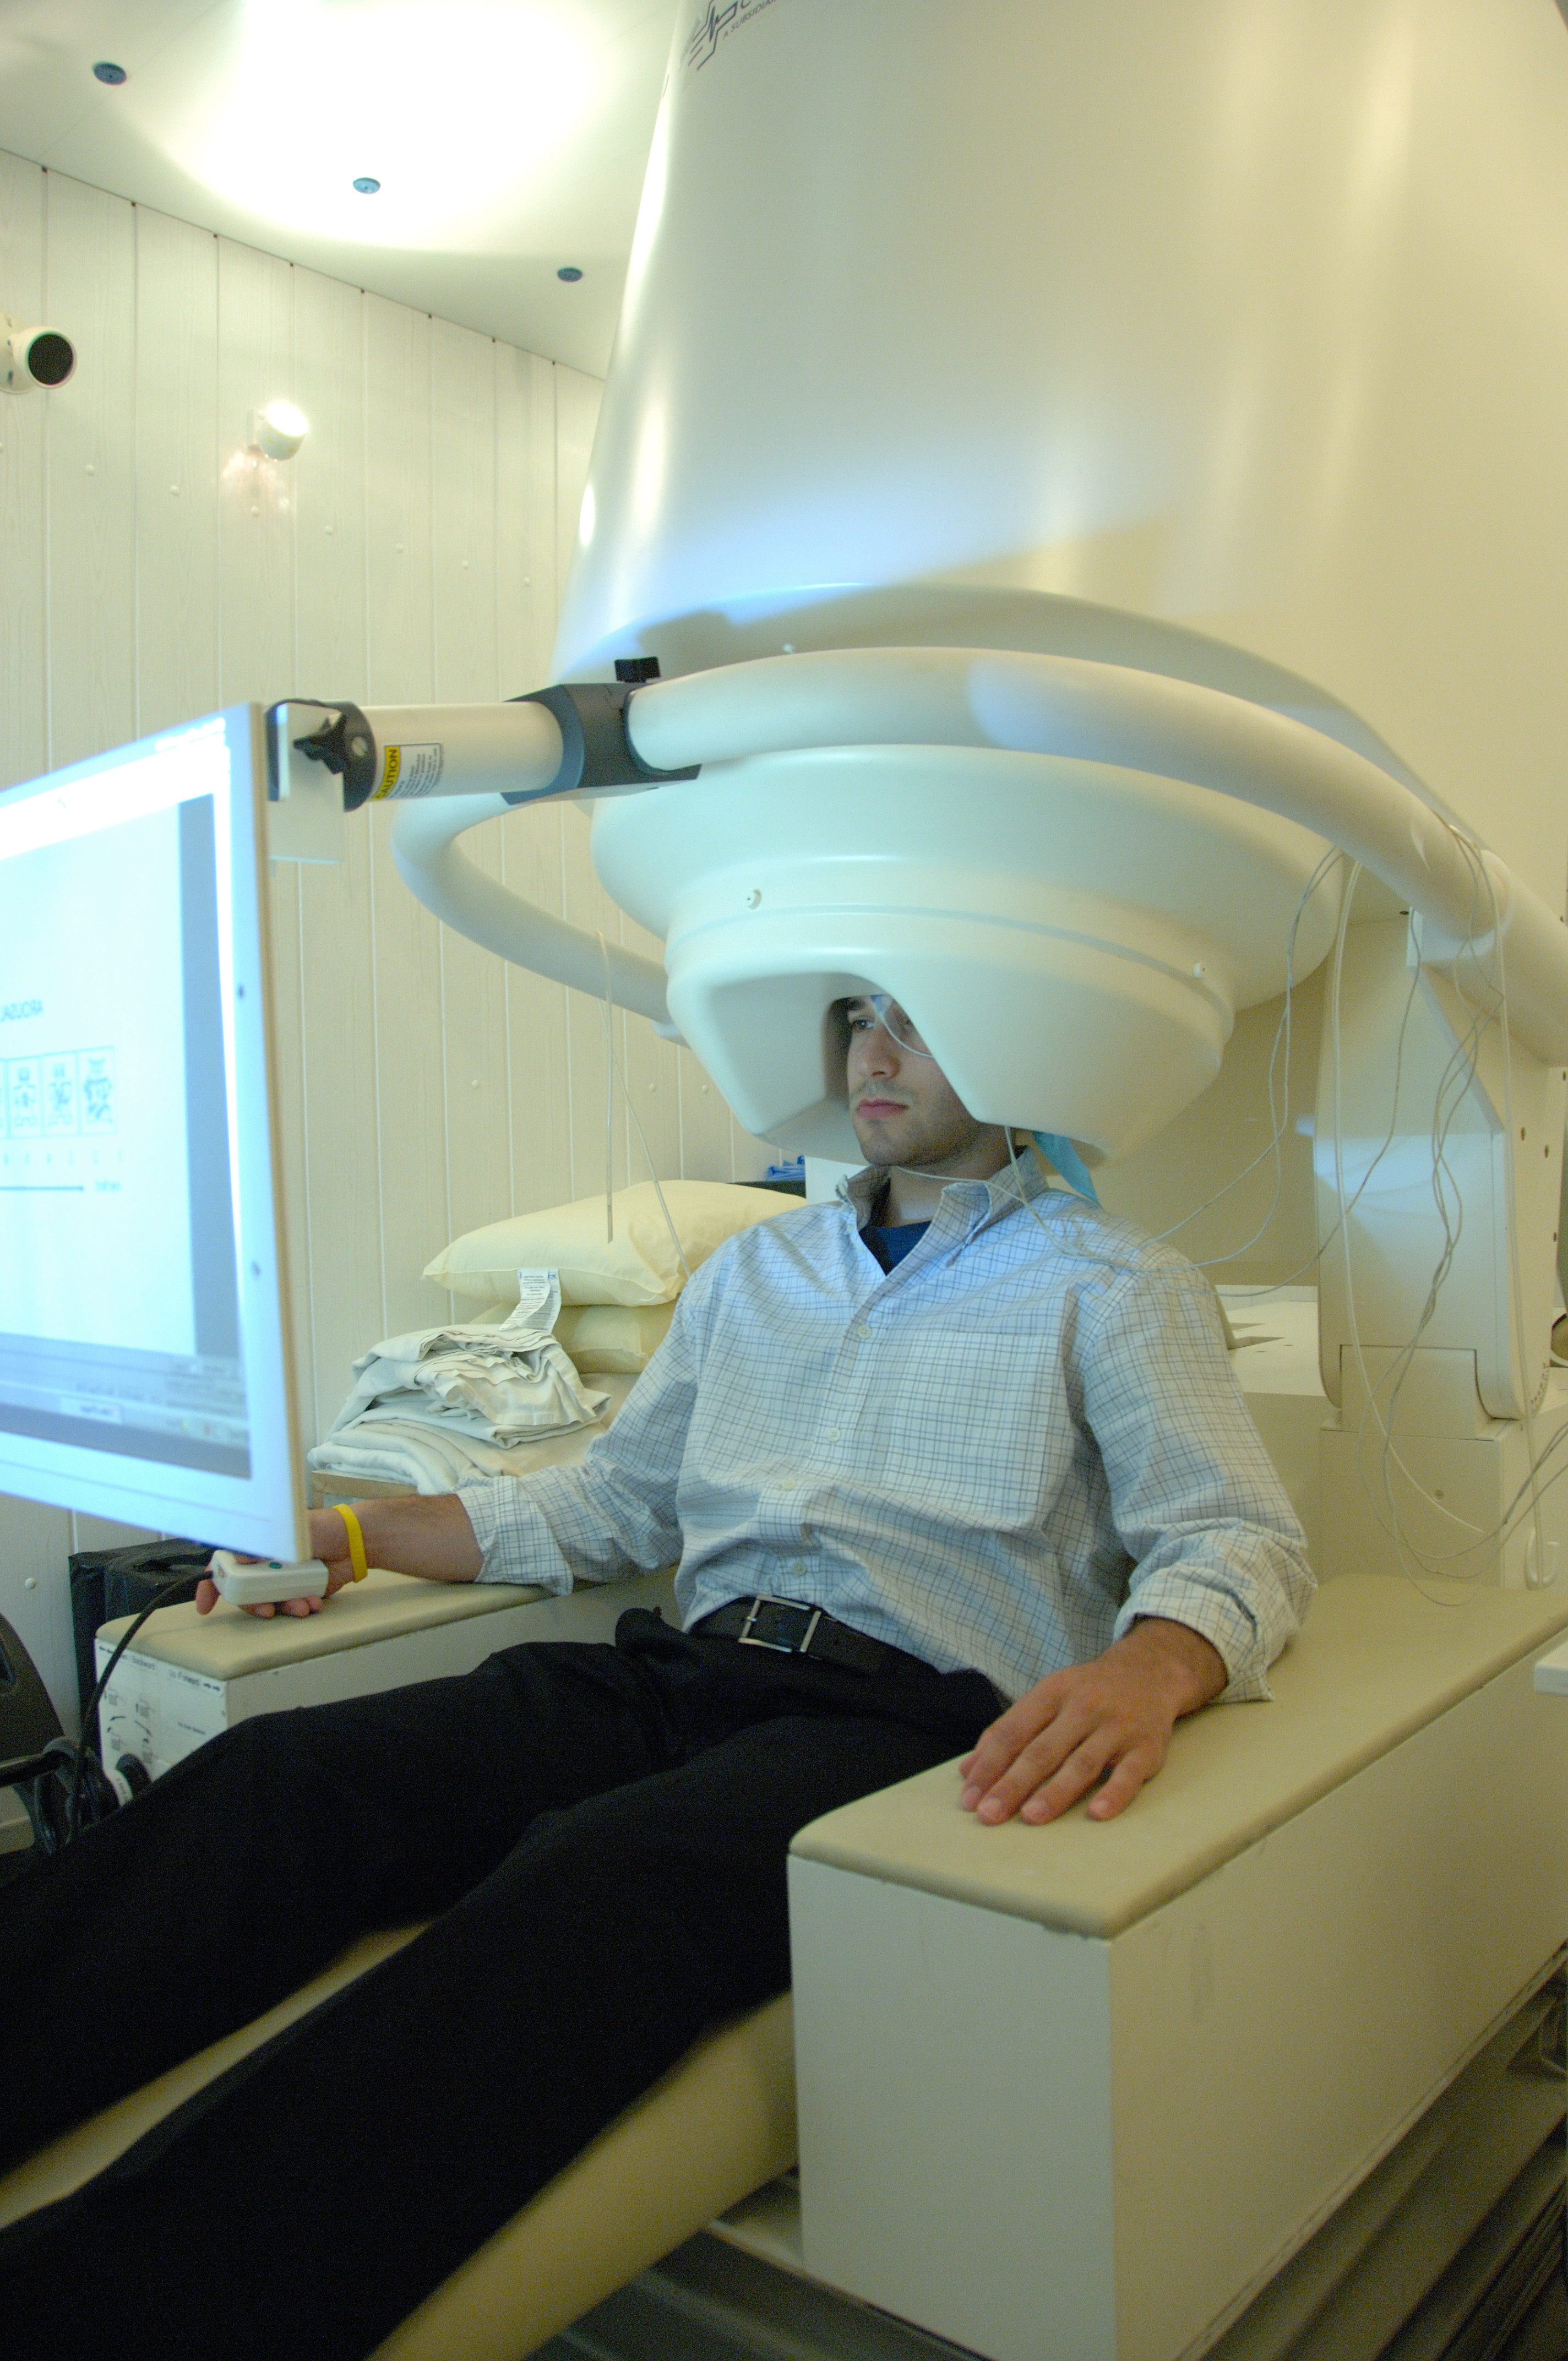
\includegraphics[height=6cm]{P2023.AIBCCSS.BrainSignals/MEG.jpg}
\end{figure}
\end{center}    

\begin{center}
    \tiny{Taken from \url{https://en.wikipedia.org/wiki/Magnetoencephalography}}
\end{center}    
\end{frame}

\begin{frame}
{\centerline{Measuring Brain Signals (6/10)}}
\begin{itemize}
    \item Positron emission tomography (PET)
\end{itemize}
\begin{figure}
    \centering
    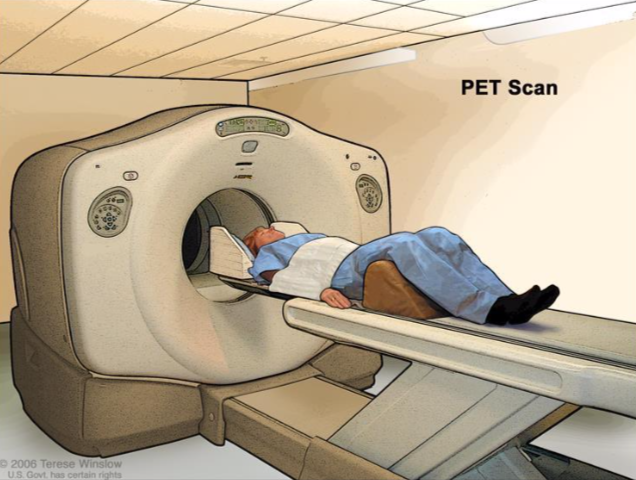
\includegraphics[height=6cm]{P2023.AIBCCSS.BrainSignals/pet.png}
\end{figure}
\begin{center}
    \tiny{Taken from \url{https://petscanhub.ie/resources/patient-information-for-pet-imaging/}}
\end{center}    
\end{frame}


\begin{frame}
{\centerline{Measuring Brain Signals (7/10)}}
\begin{itemize}
    \item Functional magnetic resonance imaging (fMRI)
\end{itemize}
\begin{figure}
    \centering
    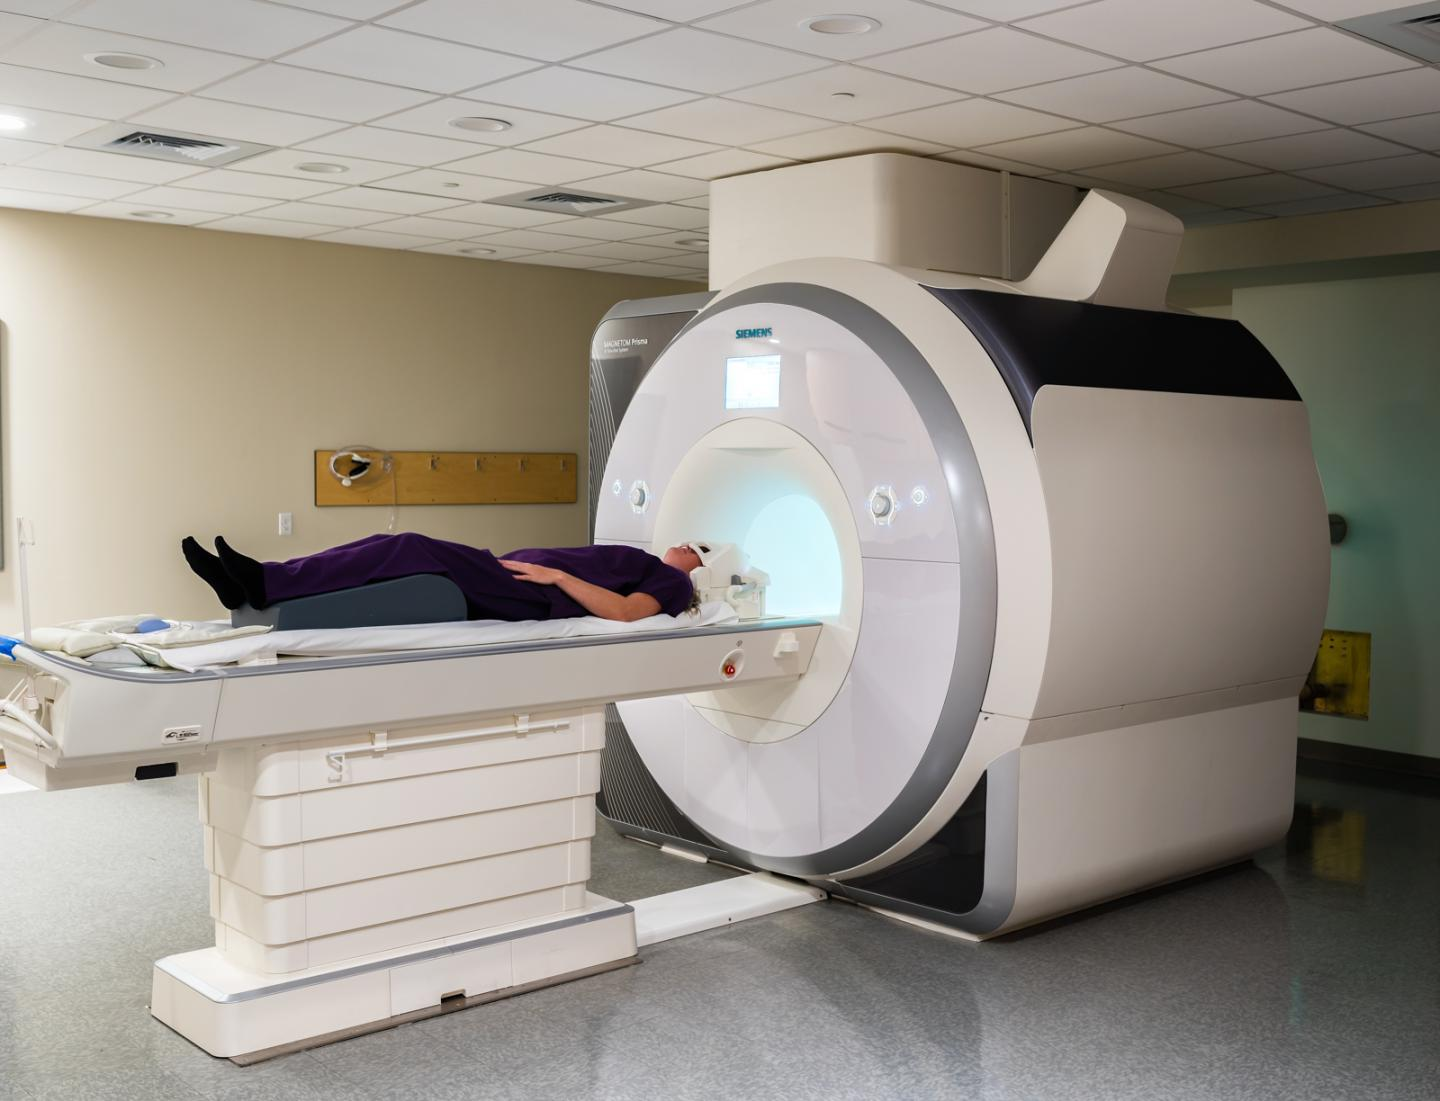
\includegraphics[height=6cm]{P2023.AIBCCSS.BrainSignals/fmri.jpg}
\end{figure}
\begin{center}
    \tiny{Taken from \url{https://www.eurekalert.org/multimedia/pub/188089.php}}
\end{center}    
\end{frame}

\begin{frame}
{\centerline{Measuring Brain Signals (8/10)}}
\begin{itemize}
    \item Functional near-infrared spectroscopy (fNIRS)
\end{itemize}
\begin{figure}
    \centering
    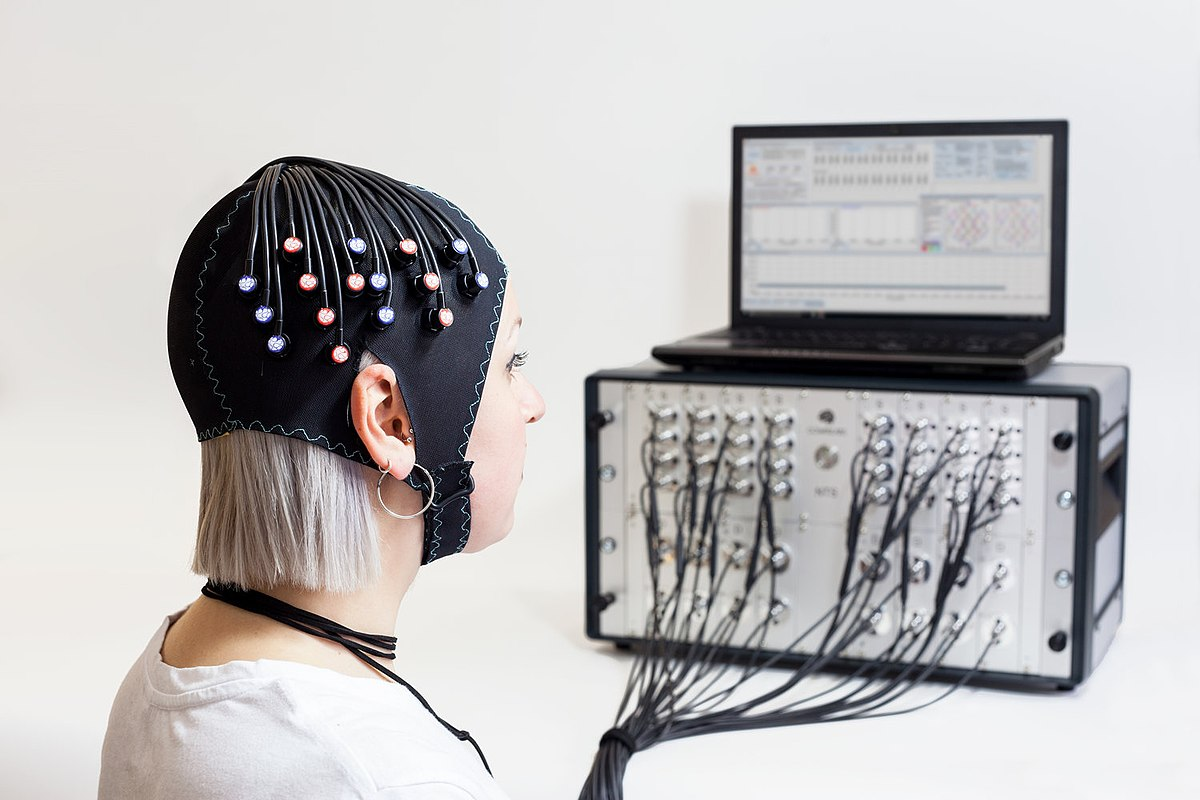
\includegraphics[height=6cm]{P2023.AIBCCSS.BrainSignals/fnirs.jpg}
\end{figure}
\begin{center}
    \tiny{Taken from \url{https://en.wikipedia.org/wiki/Functional_near-infrared_spectroscopy}}
\end{center}    
\end{frame}

\begin{frame}
{\centerline{Measuring Brain Signals (9/10)}}
\begin{itemize}
    \item Single-photon emission computed tomography (SPECT)
\end{itemize}
\begin{figure}
    \centering
    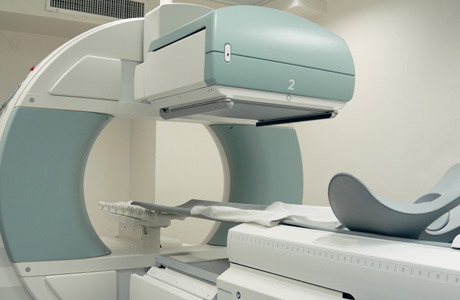
\includegraphics[height=6cm]{P2023.AIBCCSS.BrainSignals/spect.jpg}
\end{figure}
\begin{center}
    \tiny{Taken from \url{https://wa.kaiserpermanente.org/kbase/topic.jhtml?docId=acc4790}}
\end{center}    
\end{frame}

\begin{frame}
{\centerline{Measuring Brain Signals (10/10)}}
\begin{itemize}
    \item Functional ultrasound imaging (fUS)
\end{itemize}
\begin{figure}
    \centering
    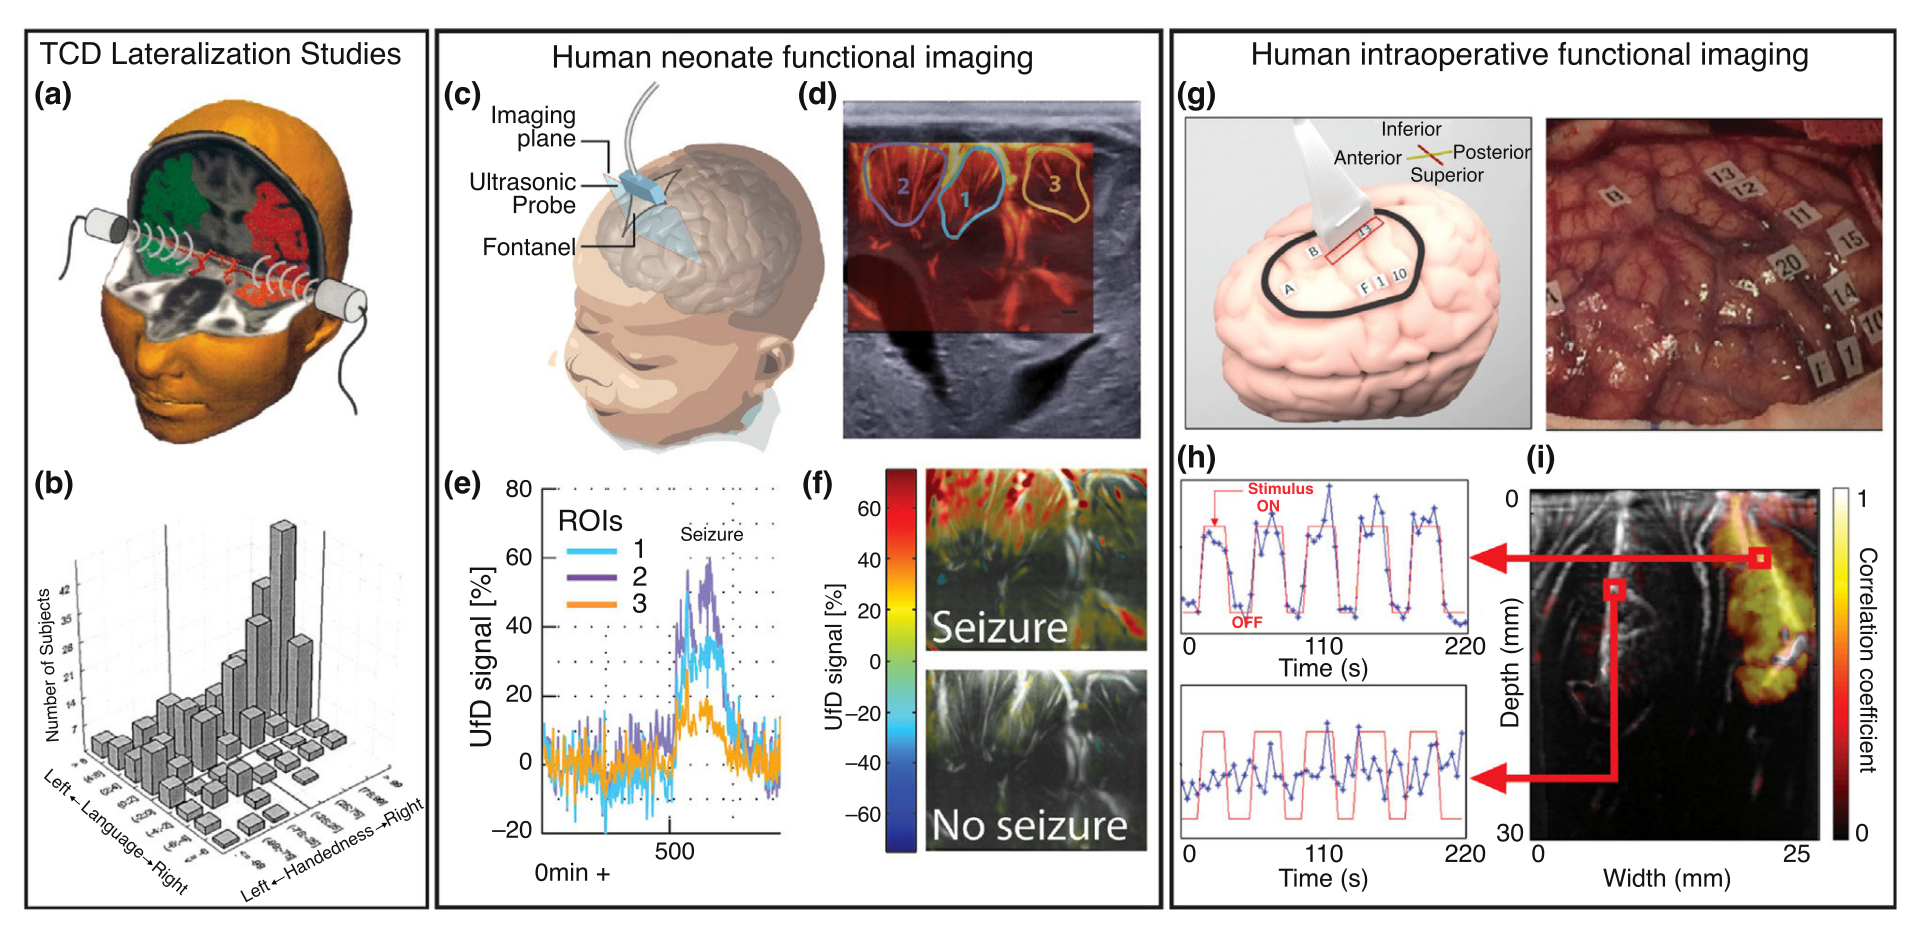
\includegraphics[height=6cm]{P2023.AIBCCSS.BrainSignals/fui.png}
\end{figure}
\begin{center}
    \tiny{Taken from \url{https://en.wikipedia.org/wiki/Functional_ultrasound_imaging}}
\end{center}    
\end{frame}

\begin{frame}
{\centerline{Inferring mental states (1/2}}
    \begin{figure}
        \centering
        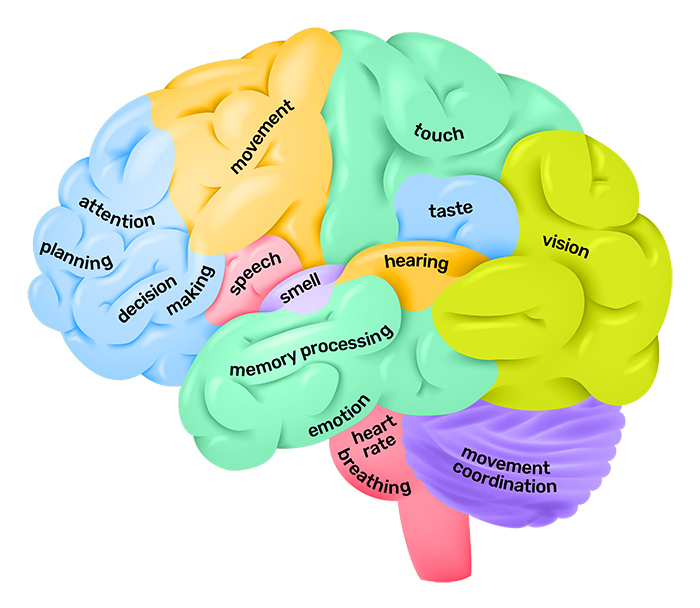
\includegraphics[height=5cm]{P2023.AIBCCSS.BrainSignals/Lobes-of-the-brain-QBI.jpg}
    \end{figure}
    \begin{center}
        \tiny{Taken from \url{https://qbi.uq.edu.au/brain/brain-anatomy/lobes-brain}}
    \end{center}
\end{frame}

\begin{frame}
{\centerline{Inferring mental states (2/2}}
    Based on brainwaves, we can find such states of human as:
    \begin{itemize}
        \item attention;
        \item emotions;
        \item memory processing;
        \item hearing;
        \item etc.
    \end{itemize}
\end{frame}

\begin{frame}
{\centerline{Collecting brain signals using EEG (1/4)}}
    \begin{itemize}
        \item Why we use EEG
     \begin{itemize}
         \item portable
         \item easier to set up
         \item not too expensive
     \end{itemize}
     \item EEG is an electrophysiological monitoring method to record electrical activity on the scalp that has been shown to represent the macroscopic activity of the surface layer of the brain underneath. 
     \item It is typically noninvasive, with electrodes placed along the scalp.
    \end{itemize}
     \begin{center}
         \tiny{Taken from \url{https://en.wikipedia.org/wiki/Electroencephalography}}
     \end{center}
\end{frame}

\begin{frame}
{\centerline{Collecting brain signals using EEG (2/4)}}
    For collecting brain signals using EEG :
    \begin{itemize}
        \item cap
        \item wired or wireless device connected to electrodes
        \item software for recording and processing EEG data
    \end{itemize}
    \begin{figure}
        \centering
        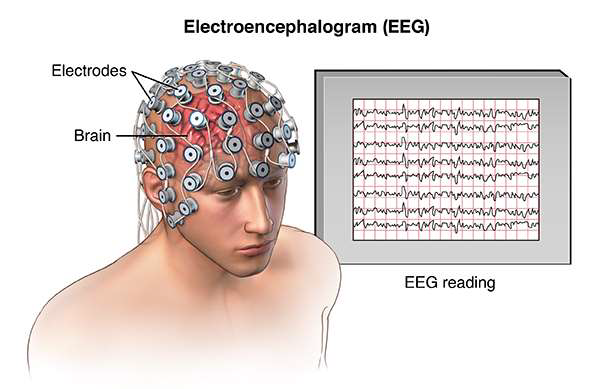
\includegraphics[width=\linewidth]{P2023.AIBCCSS.BrainSignals/EEG reading.png}
    \end{figure}
\end{frame}

\begin{frame}
{\centerline{Collecting brain signals using EEG (3/4)}}
Here known brainwaves:
\begin{itemize}
    \item $1-5$ Hz: $\delta$ (delta) wave
    \item $4-8$ Hz: $\theta$ (theta) wave
    \item $8-12$ Hz: $\alpha$ (alpha) wave
    \item $12-25$ Hz: $\beta$ (beta) wave
    \item $> 25$ Hz: $\gamma$ (gamma) wave
    \item $7,5-12,5$ Hz: $\mu$ (mu) waves
\end{itemize}
\end{frame}

\begin{frame}
{\centerline{Collecting brain signals using EEG (3/4)}}
 \begin{itemize}
     \item Neural oscillations are observed throughout the central nervous system at all levels, and include spike trains, local field potentials, and large-scale oscillations which can be measured by EEG.
     \item In general, oscillations can be characterized by their frequency, amplitude and phase.
     \item These signal properties can be extracted from neural recordings using time-frequency analysis.
 \end{itemize}
   \begin{center}
       \tiny{Taken from \url{https://en.wikipedia.org/wiki/Neural_oscillation}}
   \end{center}
\end{frame}

\begin{frame}
{\centerline{Collecting brain signals using EEG (4/4)}}
    \begin{figure}
        \centering
        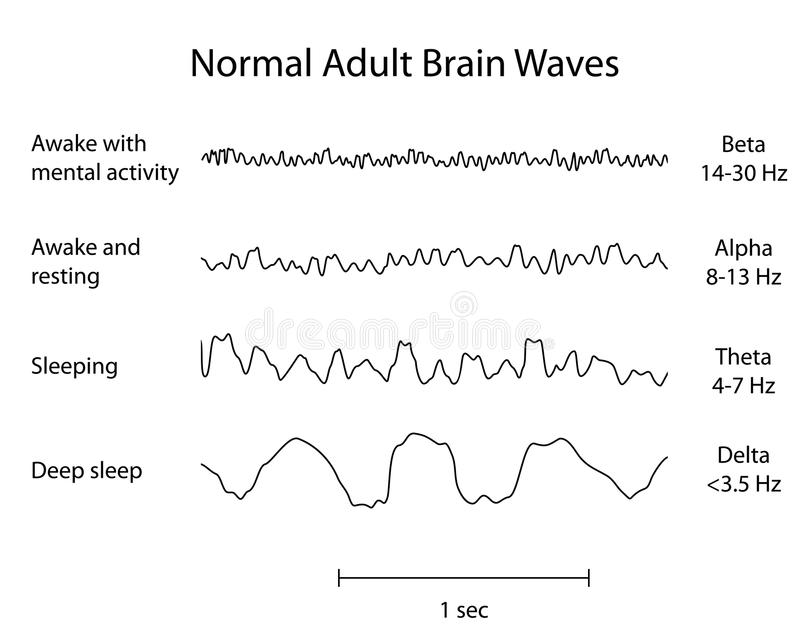
\includegraphics[height=5cm]{P2023.AIBCCSS.BrainSignals/normal-brain-waves-eeg-29444815.jpg}
    \end{figure}
    \begin{center}
    \tiny{Taken from \url{https://www.dreamstime.com/royalty-free-stock-photo-normal-brain-waves-eeg-image29444815}}
    \end{center}  
\end{frame}

\begin{frame}
{\centerline{EEG software and device}}
    For recording we use software, cap and device from Mitsar. The device is wireless, the cap is 24-channel EEG Smart BCI in which the electrodes are placed according to scheme 10-20.
    \begin{figure}
        \centering
        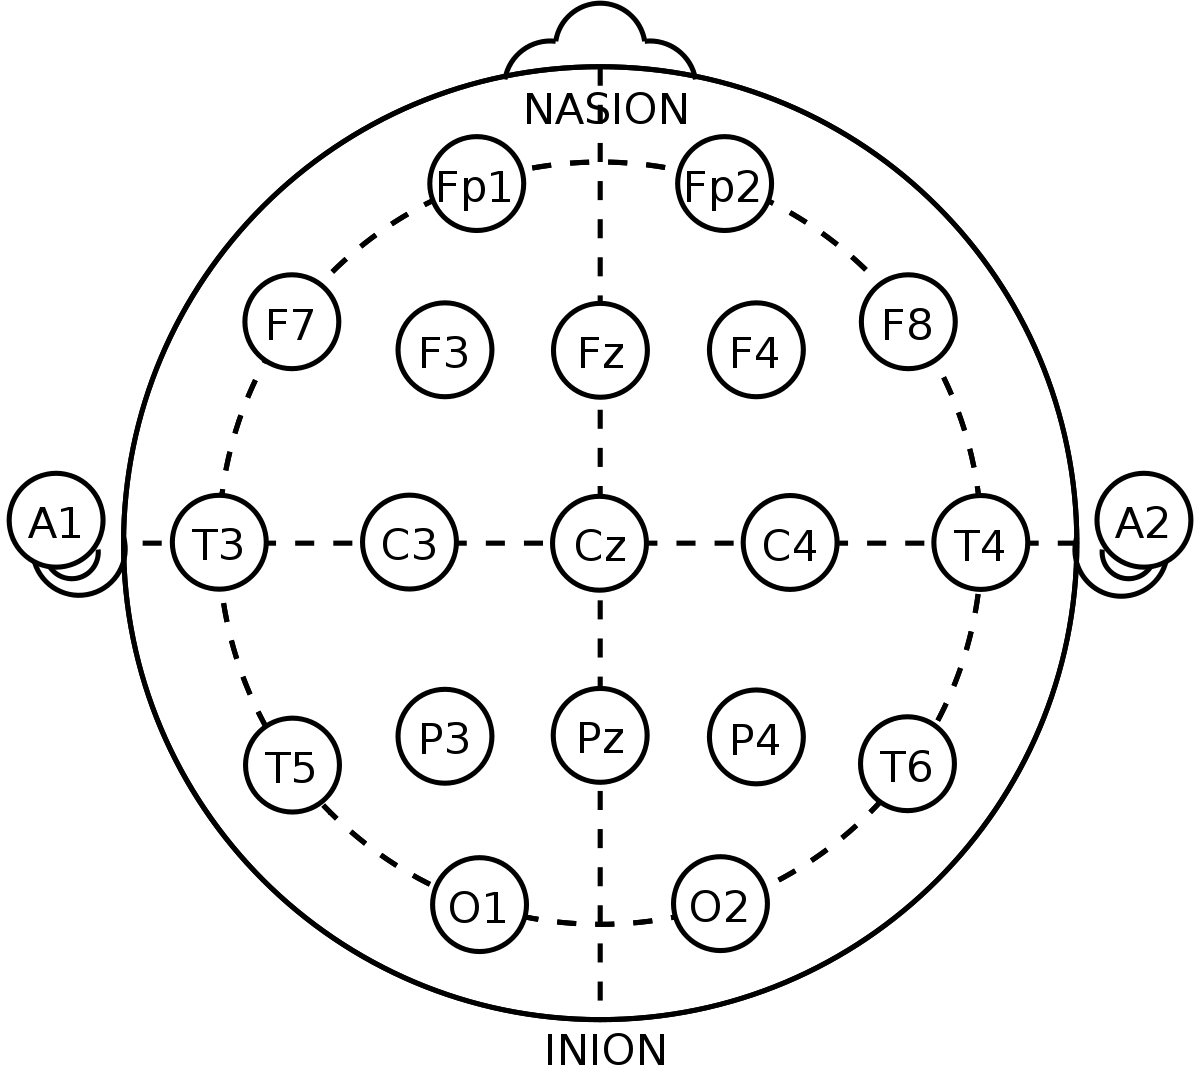
\includegraphics[height=5cm]{P2023.AIBCCSS.BrainSignals/10-20 scheme.png}
    \end{figure}
    \begin{center}
    \tiny{Taken from \url{https://en.wikipedia.org/wiki/10\%E2\%80\%9320_system_(EEG)}}
    \end{center}  
\end{frame}

\begin{frame}
{\centerline{EEG software and device that we use}}
\begin{figure}
    \centering
    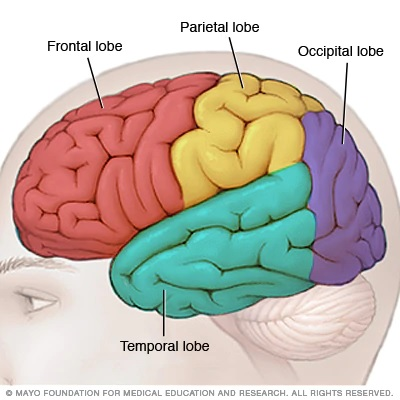
\includegraphics[height=5cm]{P2023.AIBCCSS.BrainSignals/brain_lobes.jpg}
\end{figure}
Each electrode location has a letter designating the lobe or brain region from which it reads: prefrontal (Fp), frontal (F), temporal (T), parietal (P), occipital (O) and central (C).
\begin{center}
    \tiny{Taken from \url{https://www.sv.uio.no/psi/english/research/projects/human-time-data/documents/data-lifecycle/eeg/2.\%20electrode-placement/}}\\
    \tiny{Image taken from \url{https://www.mayoclinic.org/brain-lobes/img-20008887}}
\end{center}
\end{frame}

\begin{frame}
{\centerline{Exporting EEG Data from EEG Studio}}
\href{http://www.mitsar-eeg.ru/page1.php?id=update}{EEG Studio by Mitsar} can be used for recording and processing of EEG data. You can also export the data by choosing many suitable formats: text, binary, BrainLoc, EDF, WinEEG, WinHRV, Loreta, etc. (in our purpose - the European Data Format (EDF)), where to save and what should be exported: entire examination or some individual part of examination.
\end{frame}

\begin{frame}
{\centerline{Steps in processing of EEG data}}
Trial - a test of the performance, qualities, or suitability of someone or something.

A number of event-triggered EEG trials are required for quantification, including some seconds before and after the event. The event can be external or internal (e.g., acoustic,or visual stimulation).
\end{frame}

\begin{frame}
{\centerline{Steps in processing of EEG}}

 Once the frequency band has been determined, the processing procedure consists of the following steps: 
 \begin{enumerate}
    \item bandpass filtering of each event-related trial
    \item squaring of each amplitude sample to obtain power samples
    \item averaging over all trials
    \item calculation of ERD/ERS.
 \end{enumerate}
    
\end{frame}

\begin{frame}
{\centerline{Steps in processing of EEG}}
 \begin{figure}
     \centering
     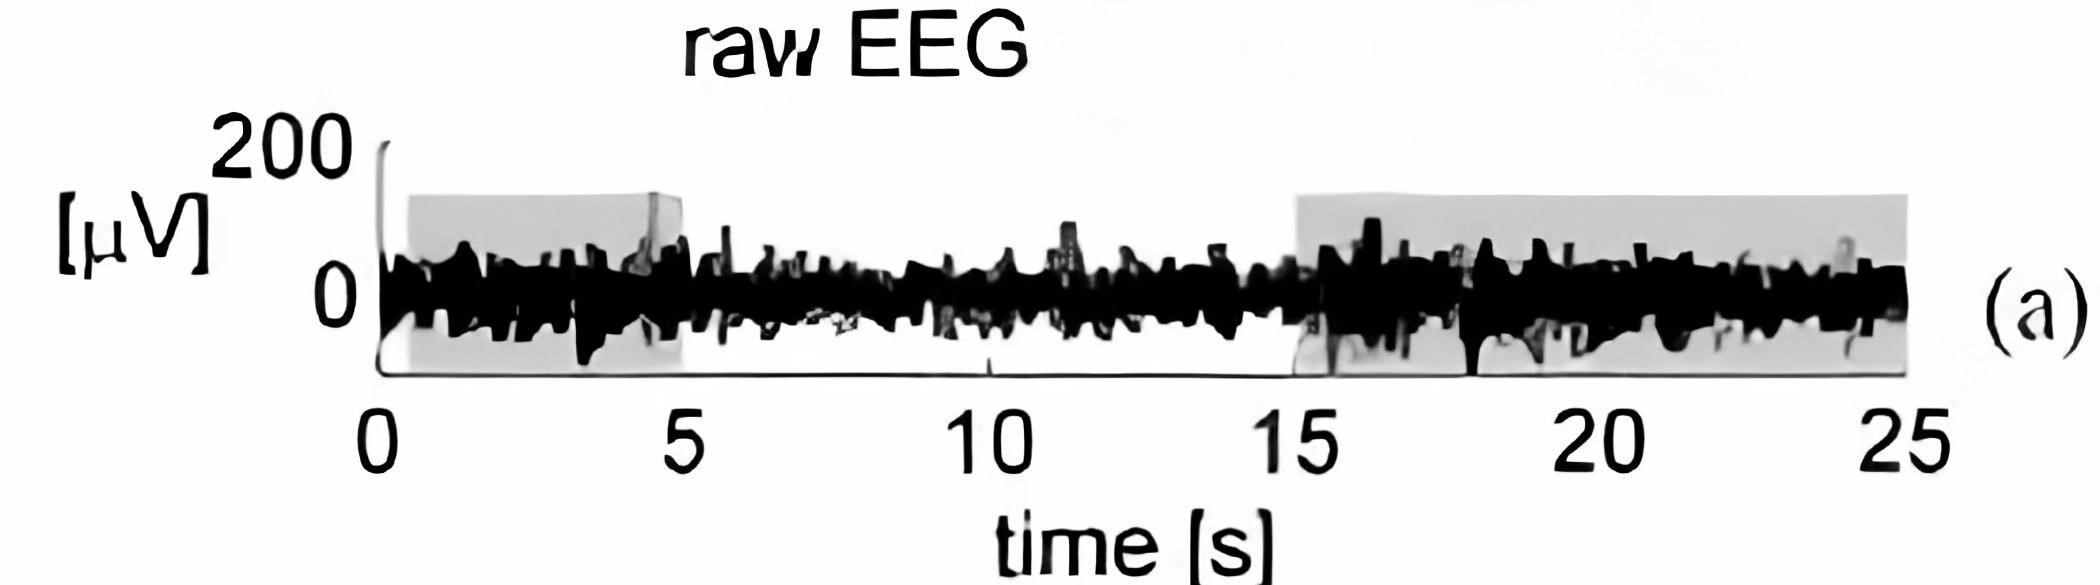
\includegraphics[width=\linewidth]{P2023.AIBCCSS.BrainSignals/Raw EEG.jpg}
     \caption{Raw EEG, on one of channels}
 \end{figure}
\end{frame}


\begin{frame}
{\centerline{Steps in processing of EEG data}}
{\centerline{Band-pass filtering}}
\begin{figure}
    \centering
    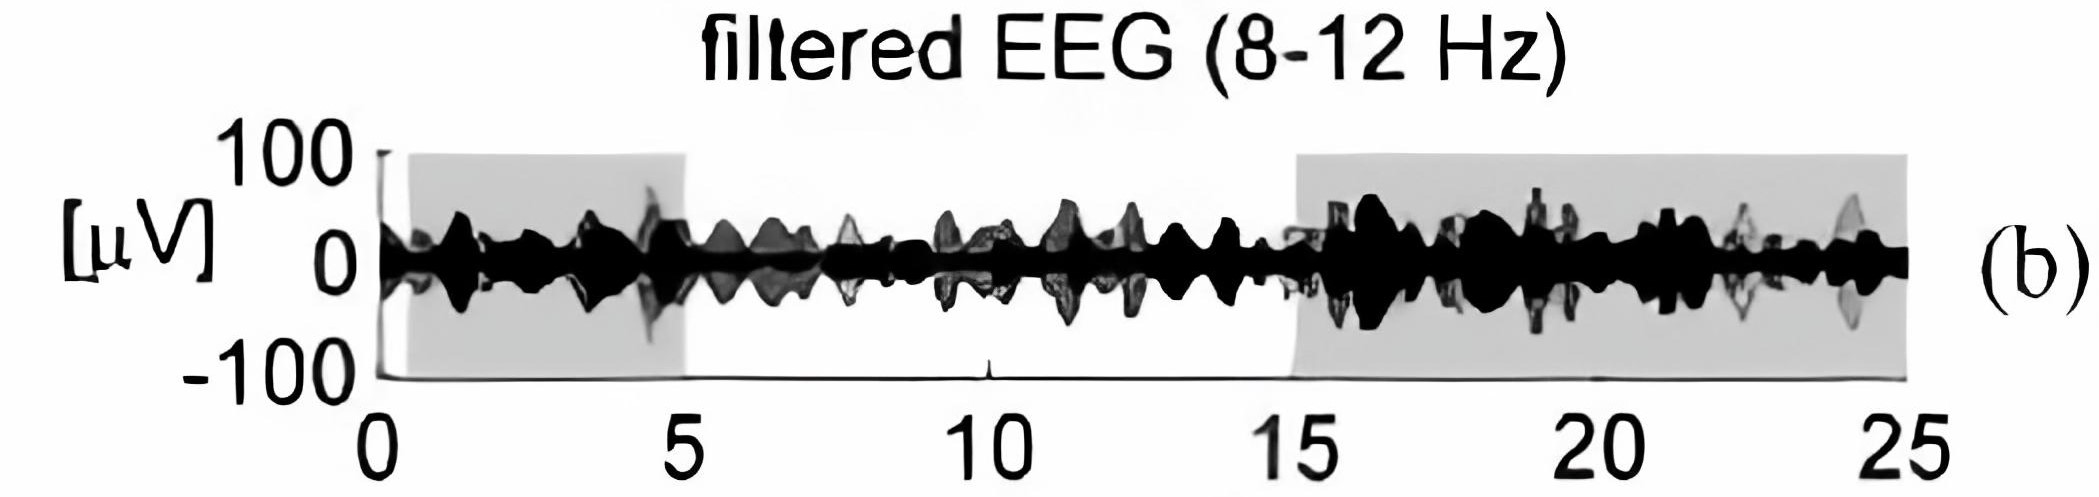
\includegraphics[width=\linewidth]{P2023.AIBCCSS.BrainSignals/banpass filtering.jpg}
\end{figure}
    An epoch is the EEG obtained in each trial under the same conditions. The EEG signals from the frontal channels were then filtered in a specific frequency band using the fast Fourier transformation.
\end{frame}

\begin{frame}
{\centerline{Steps in processing of EEG data}}
{\centerline{Band-pass filtering}}
The first step in analyzing the data is to set up the waves ranges, which can differ based on age. The variability of alpha waves in age groups has been shown to have a normal distribution ($\mu=10Hz$,$\sigma=1Hz$) and tonic changes, increasing from childhood to adulthood and then decreasing according to the formula used for the Individual Alpha Frequency(IAF).
$$IAF=11.95 - 0.053 * Age$$
\end{frame}

\begin{frame}
{\centerline{Steps in processing of EEG data}}
{\centerline{Squaring}}
    \begin{figure}
        \centering
        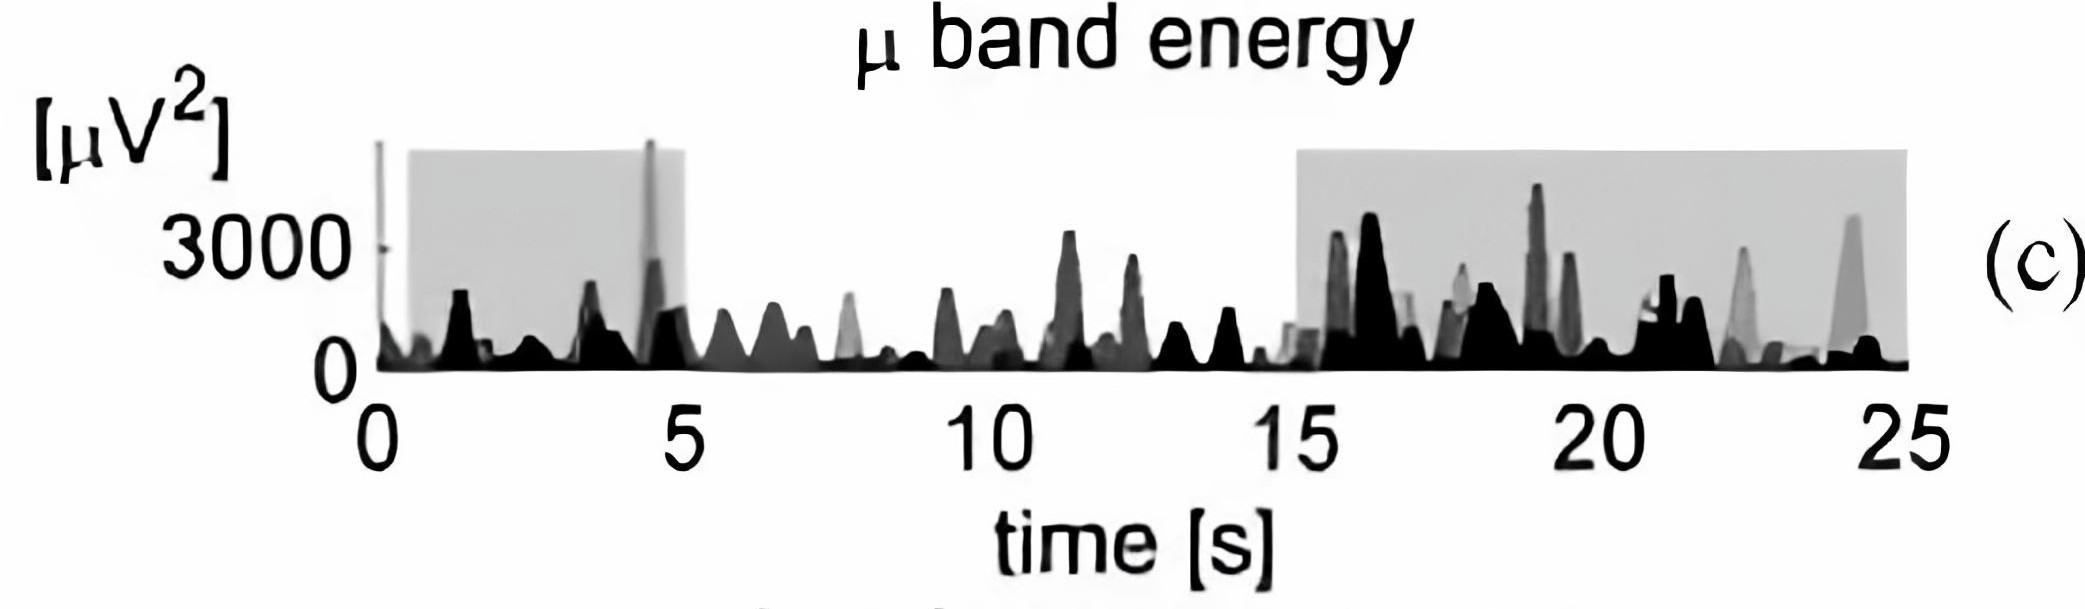
\includegraphics[width=\linewidth]{P2023.AIBCCSS.BrainSignals/squaring.jpg}
    \end{figure}
    The signal energy can be calculated by squaring the filtered EEG from each epoch.
\end{frame}

\begin{frame}
{\centerline{Steps in processing of EEG data}}
{\centerline{Averaging}}
\begin{figure}
    \centering
    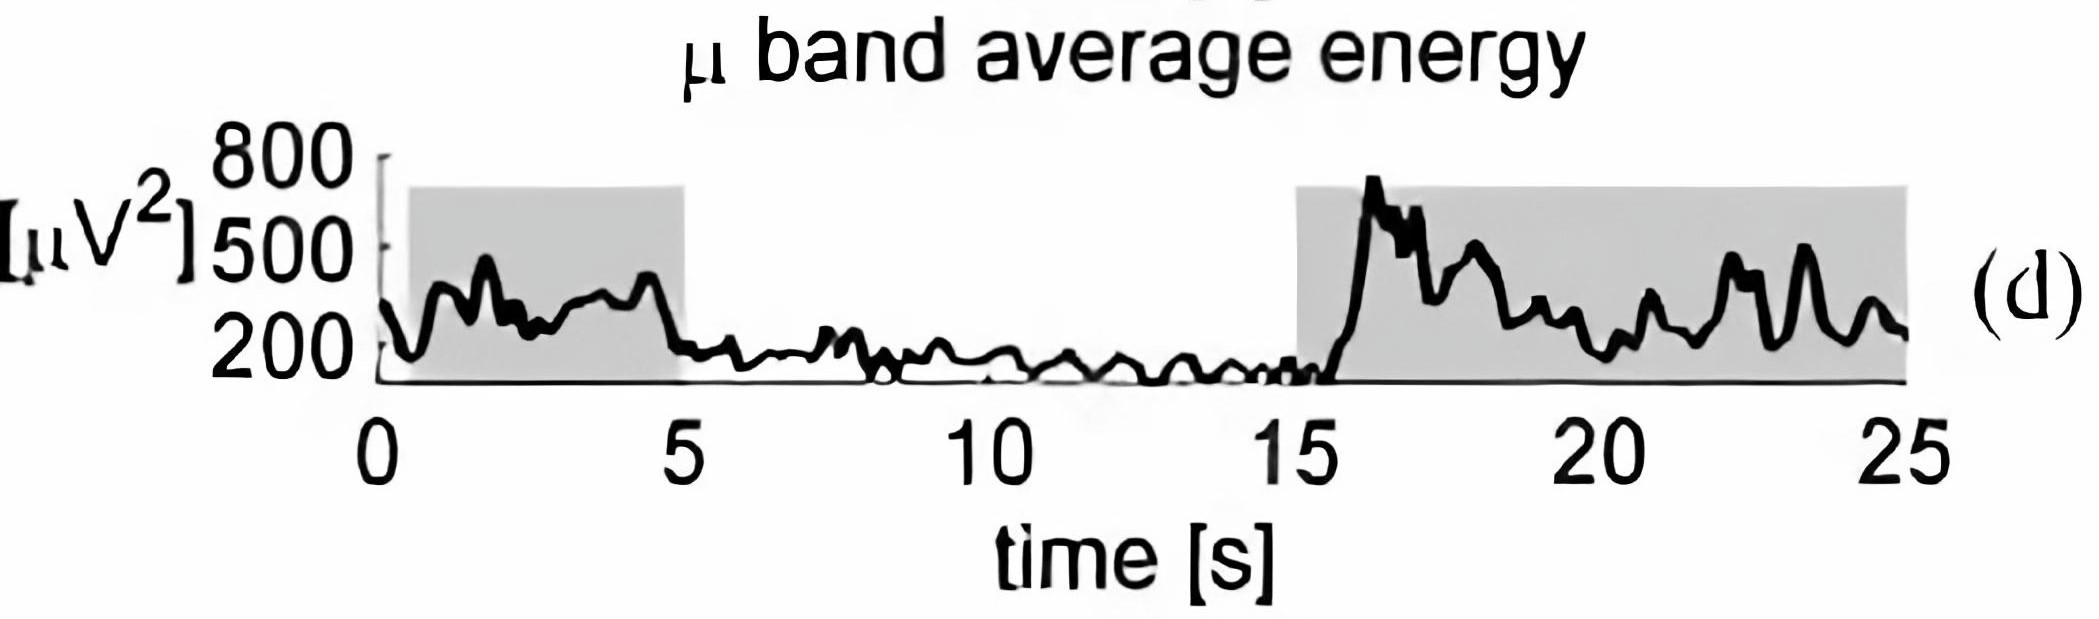
\includegraphics[width=\linewidth]{P2023.AIBCCSS.BrainSignals/averaging.jpg}
\end{figure}
    The average energy of all epochs then need to be calculated. The signal energy is used in this case to prevent the cancellation of positive and negative EEG amplitudes during the average process.
\end{frame}

\begin{frame}
{\centerline{Steps in processing of EEG data}}
{\centerline{ERD/ERS}}
    \begin{figure}
        \centering
        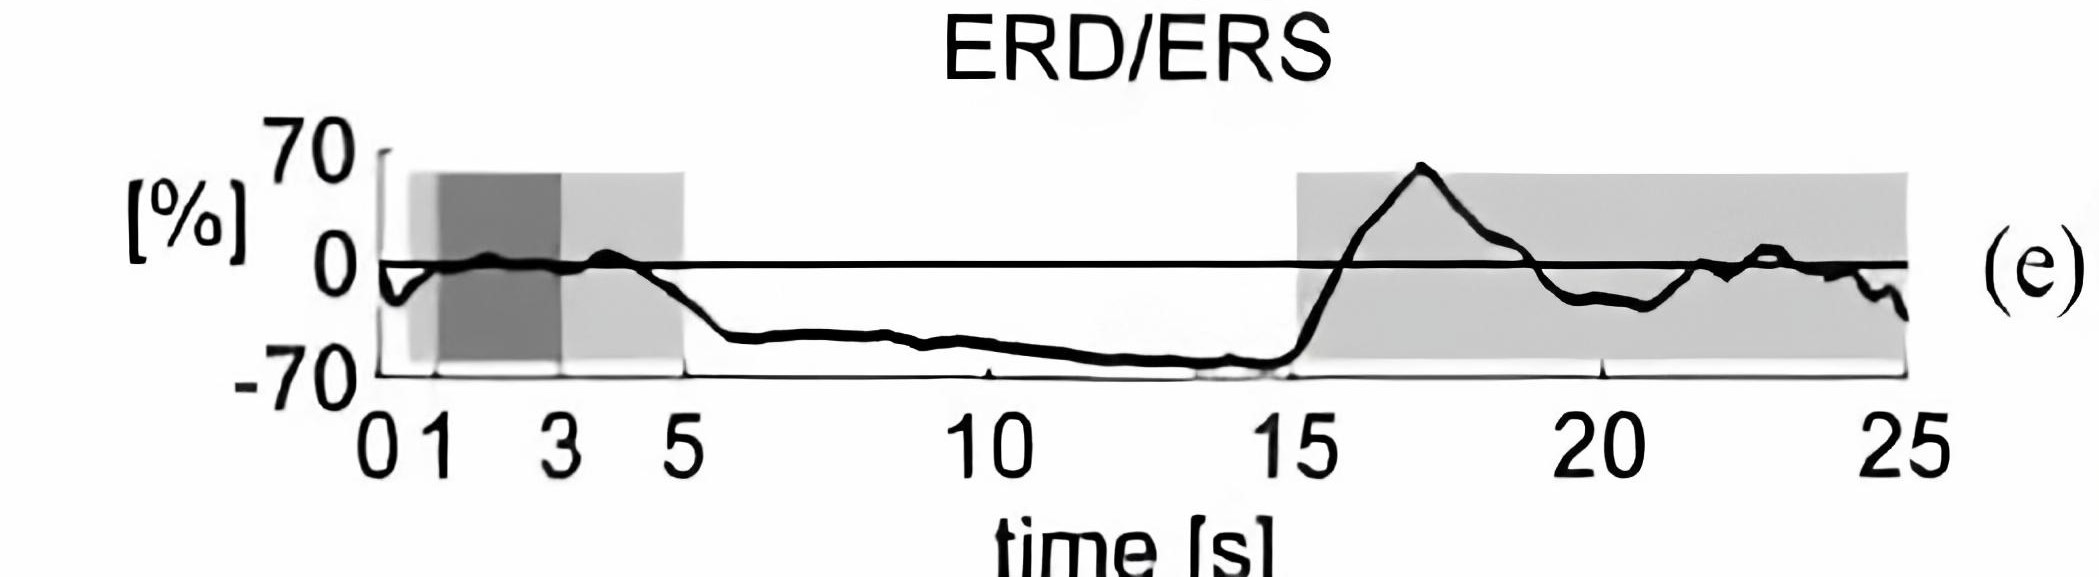
\includegraphics[width=\linewidth]{P2023.AIBCCSS.BrainSignals/ERD.jpg}
    \end{figure}
    Finally, because ERD/ERS are expressed as percentages, the average energy of a previous reference period is computed. As a result, the signal energy can be calculated in relation to the reference period.
\end{frame}

\begin{frame}
{\centerline{About the MNE}}
    MNE-Python is a subproject of the larger academic software package MNE, with the goal of developing and incorporating a set of algorithms that allow users to assemble complete data analysis pipelines covering most stages of MEG or EEG data processing. MNE-Python is a powerful EEG processing tool that provides the following features: filtering, individual component analysis, statistics, minimum normal estimation, etc. Temporal frequency analysis as well as nonparametric and connectivity studies are all possible with MNE-Python.
\end{frame}

\begin{frame}
{\centerline{About the MNE}}
    MNE analysis software selects the highest quality current distribution as a representation of all recorded currents, combining the best spatial resolution with the best temporal resolution. In addition, the frequencies of the sensor and source spaces are processed simultaneously, and anomalies can be cleaned using signal processing techniques. MNE-Python is automated with free surface power spectrum analysis tools paired with fast Fourier transformation algorithms to automatically perform a Fourier analysis of the collected data.
\end{frame}

\begin{frame}
{\centerline{Analysing EEG in Python (1/2)}}

1) with \verb|mne.io.read\_raw\_edf| read raw EEG data

2) with \verb|mne.io.concatenate\_raws| concatenate raw (if necessary)

3) with \verb|raw\_exp.info['sfreq']| get the sample frequency for main part of experiment

4) with \verb|part\_exp.pick\_channels| choose specific channels for analysis purposes

5) with \verb|mne.filter.notch\_filter| and params \verb|x=part\_exp.get\_data, Fs=sfreq, freqs=[50, 100]| filter data from AC line noise
    
\end{frame}

\begin{frame}
{\centerline{Analysing EEG in Python (2/2)}}

6) with \verb|mne.filter.filter\_data| use bandpath filtering. here we use IAF

7) with \verb|scipy.signal.spectral.stft| perform Short Time Fourier Transform

8) calculate ERD and remove outliers
    
\end{frame}

%------------------------------------------------
\begin{frame}
{\centerline{Main techniques in EEG analyzing}}
The next step is to count the number of waves in the corresponding interval. This allows us to assess brain activity at each time point. The analysis is then focused on three techniques:
\begin{itemize}
    \item ERD,
    \item Correlations of brainwaves.
    \item Mann–Whitney U-test
\end{itemize}
\end{frame}

%------------------------------------------------

\begin{frame}
{\centerline{Main techniques in EEG analyzing}}
{\centerline{ERD. Definition}}
Event-related desynchronization (ERD) reflects a decrease of oscillatory activity related to internally or externally paced events. The increase of rhythmic activity is called event-related synchronization (ERS). They represent the dynamical states of thalamocortical networks associated with cortical information processing changes.
\end{frame}

%------------------------------------------------

\begin{frame}
{\centerline{Main techniques in EEG analyzing}}
{\centerline{ERD. Calculation}}
As a result, more time-consuming work should result in a larger ERD difference between rest and programming periods. ERD is calculated using the formula shown below:
\begin{equation}
    ERD=\frac{{amplitude}_{rest}-{amplitude}_{programming}}{{amplitude}_{programming}}*100\%
\end{equation}
\end{frame}

%------------------------------------------------

\begin{frame}
{\centerline{Main techniques in EEG analyzing}}
{\centerline{Interpretation of ERD}}

\begin{figure}
    \centering
    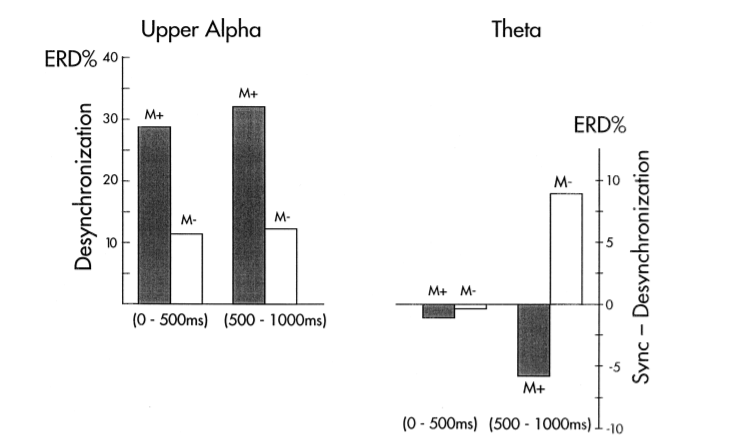
\includegraphics[height=5cm]{P2023.AIBCCSS.BrainSignals/ERD ERS.png}
\end{figure}
    \begin{center}
        ERD/ERS
    \end{center}
\end{frame}

\begin{frame}
{\centerline{Main techniques in EEG analyzing}}
{\centerline{Interpretation of ERD}}
    In a similar experiment the time course of event-related desynchronization ERD in the upper alpha and theta bands during a semantic judgment task of the type used by Klimesch et al. was analyzed separately for good (M+) and bad memory performers (M-). The results show that good memory performance (M+) is reflected by a significantly greater degree of desynchronization in the upper alpha band. The opposite is true for the theta band, where good memory performance is reflected by a greater degree of synchronization, as measured by negative ERD values.
\end{frame}

%------------------------------------------------

\begin{frame}
{\centerline{Main techniques in EEG analyzing}}
{\centerline{Correlation}}
Correlation is a statistical measure that measures how close two variables are to each other. Correlation measures the relationship, but it does not show whether x causes y or vice versa, or whether the relationship is caused by a third - perhaps unknown - factor. It can be calculated using the formula:
\begin{equation}
    r=\frac{\bar{xy}-\bar{x}\bar{y}}{\sigma_{x}\sigma_{y}}
\end{equation}
\end{frame}

\begin{frame}
{\centerline{Main techniques in EEG analyzing}}
{\centerline{Mann-Whitney U-test}}

The Mann-Whitney U-test is a statistical test can be used to assess the differences between two independent samples on the level of a characteristic measured quantitatively. It allows detecting differences in the value of a parameter between small samples. U-statistics can be calculated as:
\begin{equation}
    U=\sum_{i=1}^{n}\sum_{j=1}^{m} S(X_{i}, Y_{j})
\end{equation}
with 
\begin{equation}
    S(X,Y)=
    \begin{cases}
        1 & \text{if $Y<X$} \\
        \frac{1}{2} & \text{if $Y=X$} \\
        0 & \text{if $Y>X$}
    \end{cases}
\end{equation}
    
\end{frame}




\end{document}
